\chapter{Example Data Processing}

This chapter is partly a show case of results that are possible with
Ames Stereo Pipeline. Yet it is also a shortened guide that shows the
commands and stereo.default files used to process data. It can be hard
try to figure out what settings to start with and hopefully this will
provide starting point ideas.

\section{Apollo 15 Metric Camera}

Apollo Metric images were all taken at regular intervals, that means
that the same stereo.default can be used for all sequential pairs of
images. Apollo Metric images are some of easiest images to make stereo
data from.

The scans performed by ASU are absurdly detailed to the extent that the
film grain can be made out. This detail of information is not helpful
for the correlator, so it is recommended that subsampling the image by
4 so an actual signal is available at 1 px samplings.

Currently the tools to ingest Apollo TIFFs into ISIS are not currently
available.

\subsection{Ansgarius C}

Ansgarius C is a small crater on the west edge of the farside of the
Moon, near the equator. It is east of Kapteyn A and B.

\subsubsection*{Screenshot}

\begin{figure}[h!]
\centering
  \subfigure[{\tt 3D Rendering}]{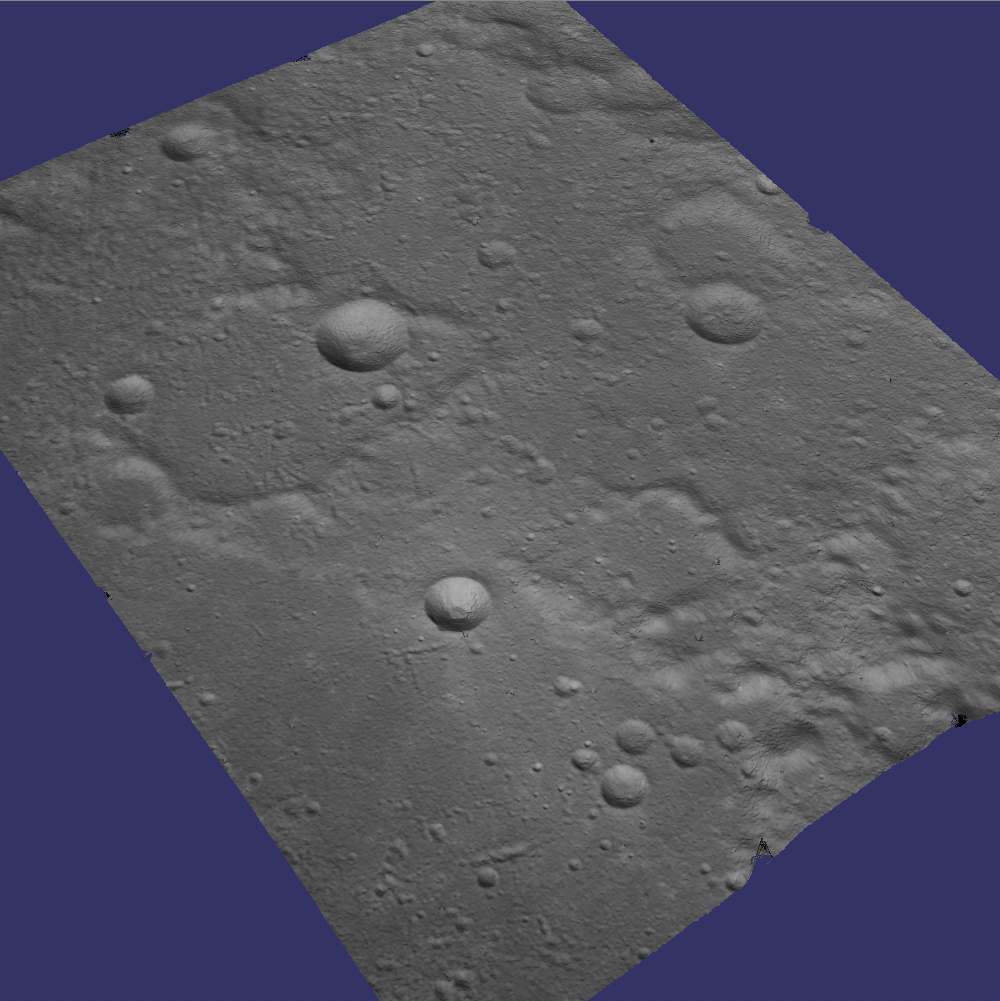
\includegraphics[width=3in]{images/examples/metric/metric_example.png}}
  \hfil
  \subfigure[{\tt KML Screenshot}]{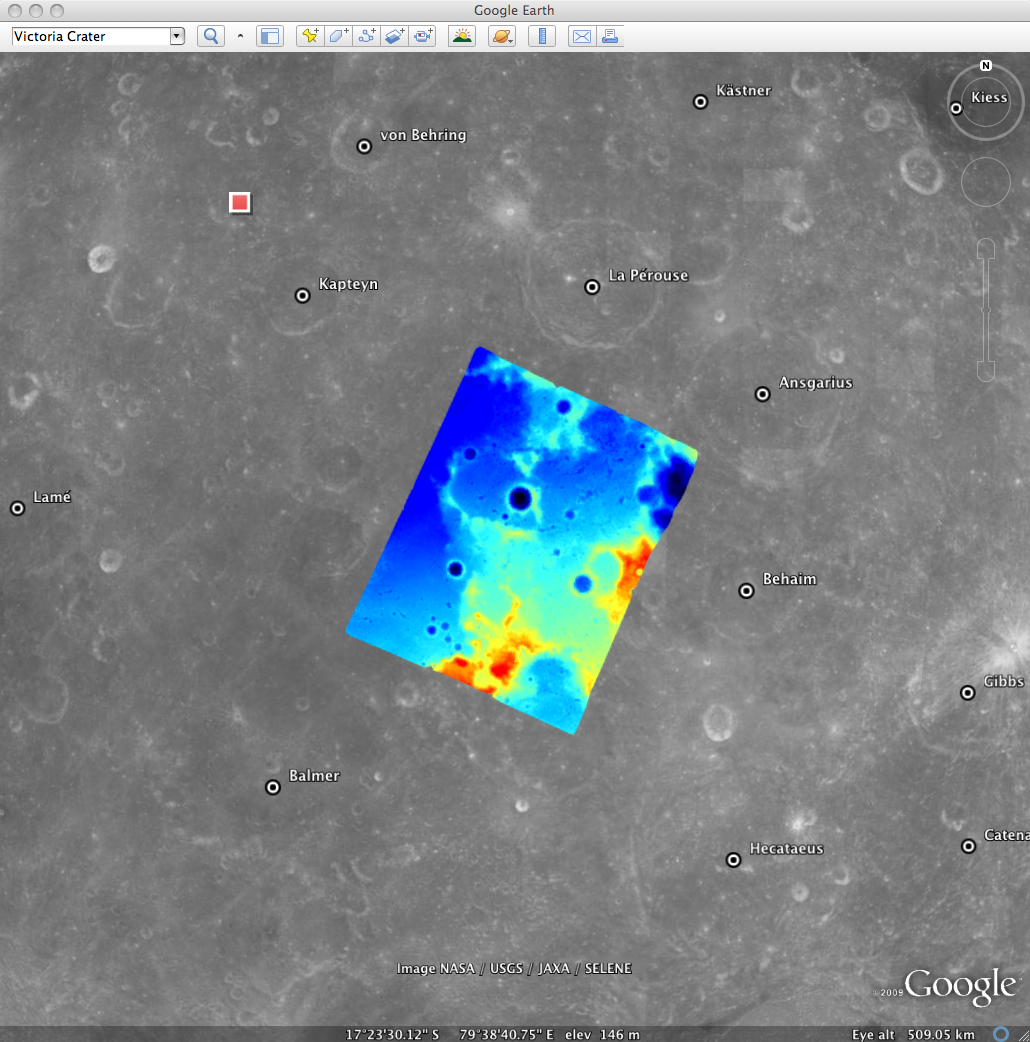
\includegraphics[width=3in]{images/examples/metric/metric_ge_example.png}}
\caption{Example output possible with Apollo Metric frames.}
\label{fig:metric_example}
\end{figure}

\subsubsection*{Commands}

\begin{verbatim}
    % Process tif files with not yet released commands %
    reduce from=AS15-M-2380.cub to=sub4-AS15-M-2380.cub sscale=4 lscale=4
    reduce from=AS15-M-2381.cub to=sub4-AS15-M-2381.cub sscale=4 lscale=4
    spiceinit from=sub4-AS15-M-2380.cub
    spiceinit from=sub4-AS15-M-2381.cub
    ipfind --max 10000 sub4*.cub
    ipmatch -i 50 -r homography sub4*.cub
    mkdir result
    stereo sub4-AS15-M-2380.cub sub4-AS15-M-2381.cub result/output
\end{verbatim}

\subsubsection*{Stereo Default}

\begin{verbatim}
    ##      PREPROCESSING      ##

    DO_INTERESTPOINT_ALIGNMENT 1
    DO_EPIPOLAR_ALIGNMENT 0
    INTERESTPOINT_ALIGNMENT_SUBSAMPLING 0
    FORCE_USE_ENTIRE_RANGE 1

    PREPROCESSING_FILTER_MODE 3
    SLOG_KERNEL_WIDTH 1.5

    ###########################    CORRELATION    ###########################

    H_KERNEL 35
    V_KERNEL 35
    SUBPIXEL_H_KERNEL 25
    SUBPIXEL_V_KERNEL 25

    H_CORR_MIN -250
    H_CORR_MAX 250
    V_CORR_MIN -70
    V_CORR_MAX 100

    SUBPIXEL_MODE 3
    DO_H_SUBPIXEL 1
    DO_V_SUBPIXEL 1

    XCORR_THRESHOLD 2.0
    CORRSCORE_REJECTION_THRESHOLD 1.4

    COST_BLUR 25
    COST_MODE 2

    ############################    FILTERING    ############################

    FILL_HOLES 1
    MASK_FLATFIELD 1

    RM_H_HALF_KERN 5
    RM_V_HALF_KERN 5
    RM_MIN_MATCHES 60 # Units = percest
    RM_THRESHOLD 3

    #############################    DOTCLOUD    ############################

    NEAR_UNIVERSE_RADIUS 0.0
    FAR_UNIVERSE_RADIUS 0.0

\end{verbatim}

\section{Cassini ISS NAC}

\subsection{Enceladus}

\subsubsection*{Screenshot}

text

\subsubsection*{Commands}

text

\subsubsection*{Stereo Default}

text

\section{Lunar Reconaissance Orbiter LROC-NA}

\subsection{Lincoln Scarp}

\subsubsection*{Screenshot}

text

\subsubsection*{Commands}

text

\subsubsection*{Stereo Default}

text

\section{Mars Global Surveyor MOC-NA}

\subsection{North Terra Meridiani}

\subsubsection*{Screenshot}

text

\subsubsection*{Commands}

text

\subsubsection*{Stereo Default}

text

\section{Mars Reconaissance Orbiter CTX}

\subsection{North Terra Meridiani}

\subsubsection*{Screenshot}

text

\subsubsection*{Commands}

text

\subsubsection*{Stereo Default}

text

\section{Mars Reconaissance Orbiter HiRISE}

\subsection{Columbia Hills}

\subsubsection*{Screenshot}

text

\subsubsection*{Commands}

text

\subsubsection*{Stereo Default}

text

\subsection{East Mareotis Tholus}

\subsubsection*{Screenshot}

text

\subsubsection*{Commands}

text

\subsubsection*{Stereo Default}

text

\subsection{North Terra Meridiani Crop}

\subsubsection*{Screenshot}

text

\subsubsection*{Commands}

text

\subsubsection*{Stereo Default}

text

\section{MESSENGER MDIS}

This a proof of concept showing of the strength of building on top of
ISIS. MDIS data is not a goal for the designers but it does have a
camera model in ISIS. This alone means that it too can be processed by
the Ames Stereo Pipeline.

For future mappers it is suggested checking out Mercury Flyby 3 data
which was not available at the time of this writing. Flyby 3 and Flyby
2 seem to have covered some of the same terrain with the narrow angle
camera.

\subsection{Wide Angle on flyby 2}

Like most imagery coming from spacecraft that are currently not in
orbit with their target, it is very hard to find good stereo
pairs. This is taken from a single flyby from the same camera seconds
apart. It should also be noted that this pair is taken from different
wave lengths as well \emph{(The letter at the end of the file
  designates the current filter being used on the wide angle
  camera)}. Unfortunately theres not enough of a perspective change to
make anything other than the spherical surface.

\subsubsection*{Screenshot}

\begin{figure}[h!]
  \begin{center}
  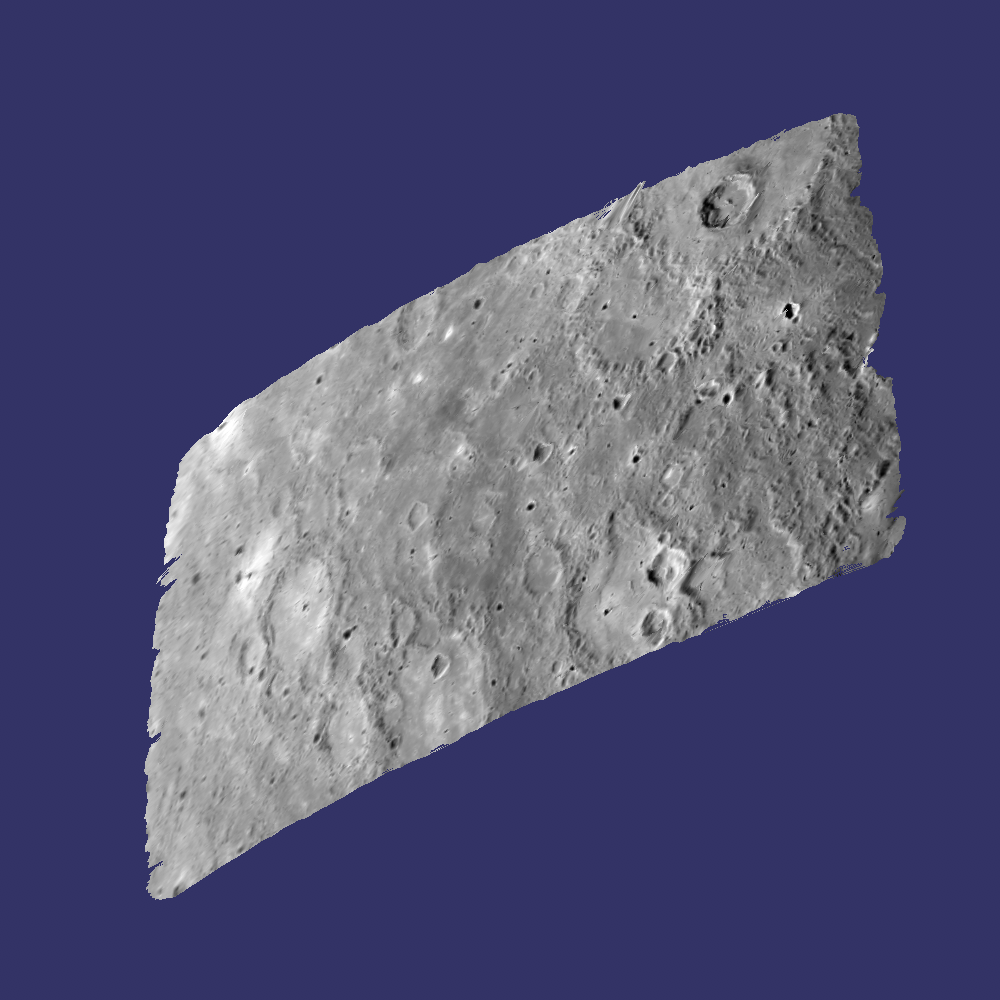
\includegraphics[width=5in]{images/examples/mdis/mdis_wide_example.png}
  \end{center}
  \caption{ A rough attempt at MDIS imagery }
  \label{fig:mdis_attempt}
\end{figure}

\subsubsection*{Commands}

\begin{verbatim}
    mdis2isis from=EW0108825359A.IMG to=EW0108825359A.cub
    mdis2isis from=EW0108825379C.IMG to=EW0108825379C.cub
    spiceinit from=EW0108825359A.cub
    spiceinit from=EW0108825359C.cub
    ipfind --max 10000 *.cub
    ipmatch -i 10 -r homography *.cub
    mkdir result
    stereo EW0108825359A.cub EW0108825379C.cub stereo/output
\end{verbatim}

\subsubsection*{Stereo Default}

\begin{verbatim}
    ##      PREPROCESSING      ##

    DO_INTERESTPOINT_ALIGNMENT 1
    DO_EPIPOLAR_ALIGNMENT 0
    INTERESTPOINT_ALIGNMENT_SUBSAMPLING 0
    DO_INDIVIDUAL_NORMALIZATION 1
    FORCE_USE_ENTIRE_RANGE 0

    PREPROCESSING_FILTER_MODE 2
    SLOG_KERNEL_WIDTH 1.5

    ###########################    CORRELATION    ###########################

    H_KERNEL 25
    V_KERNEL 25
    SUBPIXEL_H_KERNEL 19
    SUBPIXEL_V_KERNEL 19

    H_CORR_MIN -10
    H_CORR_MAX 10
    V_CORR_MIN -2
    V_CORR_MAX 2

    SUBPIXEL_MODE 2
    DO_H_SUBPIXEL 1
    DO_V_SUBPIXEL 1

    XCORR_THRESHOLD 2.0
    CORRSCORE_REJECTION_THRESHOLD 1.3

    COST_BLUR 5
    COST_MODE 0

    ############################    FILTERING    ############################

    FILL_HOLES 1

    RM_H_HALF_KERN 5
    RM_V_HALF_KERN 5
    RM_MIN_MATCHES 60 # Units = percent
    RM_THRESHOLD 3

    #############################    DOTCLOUD    ############################

    NEAR_UNIVERSE_RADIUS 0.0
    FAR_UNIVERSE_RADIUS 0.0

\end{verbatim}
